{\noindent \normalsize \bf Dear VLDB Chairs and Referees: }

\vspace{.5em}

We thank the reviewers for the helpful feedback on our paper. 
We addressed all of the concerns and included references to the revised text. 
To remind the reviewers, \sys studies techniques for iterative data cleaning before Machine Learning model training.
In summary, the major revisions are:

\begin{enumerate}
\item We included new results on a dataset of movie plot descriptions from IMDB with real errors. We also clarified that the experiment that was previously in the paper was real as well. Accordingly, we have re-organized the experiments section to describe these applications in more detail~(Section \ref{real-errors}).

\item As the reviewers suggested, we have revised Section \ref{intro} and Section \ref{background} to be more accessible to a general audience. We expanded our discussion about the convergence problem in the introduction and revised our background section to illustrate this in the context of one of our experimental datasets.

\item We further revised the presentation of the sampling component of \sys. We clarified that ``sampling'' means the process of selecting a new batch of data to be cleaned (new Section \ref{dist-samp}). 

\item We have also clarified the relationship between \sys and Active Learning. Active Learning studies the problem of acquiring the most valuable labels for unlabeled data. On the other hand, \sys studies select the most valuable data to clean in a dirty dataset (Section \ref{background}). 

\end{enumerate}

\subsection*{Meta Review Details} 

\noindent\noindent \textbf{This paper addresses an interesting problem: interactively cleaning data to improve ML models. Reviewers are happy with the theoretical results on convergence and the solution proposed. One important concern is the lack of experiments on real dirty data. Hopefully, this can be addressed in a revision.}

\vspace{0.5em}

We thank the reviewers for insisting on an evaluation of \sys with real data and errors. We believe that benchmarking data cleaning on real use cases is an important issue, and accordingly, we have revised our experiments (Section \ref{eval}) to include an additional experiment on a real dataset with real errors. 

This new experiment explores a dataset of movie descriptions from the Internet Movie Database (IMDB). 
Each movie has a title, a 1-2 paragraph plot description, and a list of categories.
We train a classifier on this data that predicts whether a movie is a ``Horror'' movie or a ``Comedy'' from the plot description and the title.
However, since much of this data is user-contributed, the categories listed are often dirty with redundant and sometimes conflicting tags.
There are also numerous examples of parsing artifacts in the plot description.
We clean this dataset by cross-referencing the IMDB dataset with a cleaner, curated dataset of movies from Yahoo.

This dataset also shows experimental evidence for systematic bias.
Horror movies were more likely to be erroneously tagged, and consequently, a classifier trained on the dirty data favored ``Comedy'' predictions. 
On the dirty dataset, the prediction precision of the classification model for Horror movies was only 29\%.
The precision improved to 74\% after data cleaning.

In our original submission, we did include an experiment performed on real data with real errors. 
We apologize that the writing was unclear. We have revised the experiments to move the real datasets up-front, and expanded our discussion of the datasets, challenges, and results~(Section \ref{real-errors}).

\subsection*{Review 1 Details} 

\noindent\textbf{R1.1: I'm not fully convinced that mixed dirty and clean data can be even worse than no cleaning. It would be helpful to show experimental support from the beginning for this and clarify whether this holds in general or only applies to certain models.}

\noindent Any aggregate over multiple populations of data is susceptible to Simpson's Paradox, and this problem has affected several high-profile studies (e.g.,~\cite{bickel1975sex, charig1986comparison}).
One of the most famous examples of Simpson's paradox occurred during an analysis of UC Berkeley Admissions in 1975~\cite{bickel1975sex}: a study found that women were statistically significantly less likely than men to be admitted to UC Berkeley; however, further analysis revealed that women were just more likely to apply to selective departments, and there no significant gender bias in any particular department. 
Partial data cleaning results in two distinct populations of data (clean and dirty), and a model trained on the mix may learn correlations that do not exist in either population. 
We have added a new paragraph to the introduction to clarify the relevance of Simpson's Paradox to data cleaning and expanded a conceptual example in which this occurs.
The background section further describes how such a scenario arises during iterative data cleaning.

We believe that this problem is important for two reasons: (1) any model trained on a mix of dirty and clean data is theoretically affected, but the analyst could not know this in advance without actually cleaning the dataset, (2) even if this is not a problem, the particular algorithm converges slowly in practice (Section \ref{real-errors}).
The magnitude of the actual bias depends on the data distribution, the amount of data cleaning, and particulars of the statistical model.
A tool like \sys provides a guarantee against this bias whether or not it actually occurs.

\vspace{0.5em}

\noindent\textbf{R1.2: The algorithm is based on the assumption that we have to do sampling. Why is sampling necessary? Especially that the experimental data sets and examples are not big. If we do not do sampling, how would the solution change? Also, why is the sample potentially stochastic?}

\noindent Any iterative or progressive data cleaning framework will clean data in small batches in each iteration. 
If we do not do sampling, the solution will reduce to a non-iterative data-cleaning framework, which presents the entire data for the analyst to clean.
The sampling algorithm in \sys is the procedure to select which data to present based on the current model and previously cleaned data.
While the selection of dirty records has to be stochastic, since a deterministic prioritization may lead to excluding certain data from cleaning, we show how this approach can be integrated with deterministic rules to select data expected to be dirty~(Section \ref{det}).

\vspace{0.5em}

\noindent\textbf{R1.3 Why does the paper focus on convex loss functions? Which theorems would not hold w/o this assumption?}

\noindent We had chosen to address this point in our technical report~(see Appendix C in \cite{activecleanarxiv}). We have now added an intuitive explanation to the revision (Section \ref{sgd}):

\emph{Gradient descent techniques still apply to non-convex losses as they are widely applied in graphical model inference and deep learning. Instead of converging to a global optimum,
they converge to a locally optimal value. However, there is a dependence on the initialization.
In the non-convex setting, ActiveClean will converge to the closest locally optimal value to
the dirty model (which is how we initialize). Because of this, it is harder to reason about
the objective quality of the results and to define accuracy.
 Different initializations may lead to different local
optima, and thus, introduces a complex dependence on the
initialization with the dirty model.}

\vspace{0.5em}

\noindent\textbf{R1.4 For cleaning, is it through cleaning on random samples, or by cleaning rules? My understanding is that it is the former but why not the latter?}

\noindent \sys cleans a batch of data in each iteration. 
There are two main issues: (1) which data are in the batch and (2) how to clean the batch. 
For (1), \sys is fully compatible with rule-based techniques to select dirty data that violate these rules (Section \ref{rule-det}).
We assume that (2) is given to us in the form of a user-defined function that is implemented either with software or a manual action by the analyst (Section \ref{dmodel}). 
Given a dirty batch of data this function returns a cleaned batch of data (if a record is not dirty, it just passes through).
One could use also the same rules to synthesize repairs on the batches as in~\cite{DBLP:journals/pvldb/YakoutENOI11}.

\vspace{0.5em}

\noindent\textbf{R1.5 The experimental data are in a sense synthetic (clean data are corrupted), which is very disappointing. It will be much more convincing to show on at least one REAL data set how the dirty data can lead to bad models and how the proposed solutions can help.}

\noindent We greatly value this suggestion and have expanded our experiments to include an additional real dataset.
Section \ref{real-errors} describes two real scenarios, a movie dataset from IMDB and a medical dataset from ProPublica, and how these use cases can be addressed by \sys.

The first scenario is an automatic content tagging problem where a classifier categorizes movies from plot descriptions.
Each movie has a title, a short 1-2 paragraph plot description, and a list of categories, and the goal is to train a model to predict whether a movie is a ``Horror'' or ``Comedy'' from the description and title. 
This data is user-contributed, and the category list is very dirty, with redundant, spurious, and conflicting tags.  
Thus, we used a cleaner reference dataset from Yahoo Movies and performed simple entity resolution to match movies together, and imported the Yahoo dataset's categories to the IMDB dataset when possible.
``Horror'' movies were more likely to have incorrect category tags, and thus, the prediction accuracy of the model was greatly affected. 
We applied \sys to select the movies were the most valuable to import (Section \ref{imdb}). 

The second scenario resembles a fraud detection problem where a classifier determines whether corporate medical donations are suspicious.
In this dataset, company names were often inconsistently represented in the data, e.g., Pfizer Inc., Pfizer Incorporated, Pfizer.
Furthermore, donation records were often inconsistently flagged, e.g. Suspicious, Review, Disallowed.
This dataset has a systematic bias because records that were suspicious were more likely to have an inconsistent flagging attribute and inconsistencies in the company name.
We applied \sys to select the most valuable records to check and repair when possible (Section \ref{exp:dfd}). 

\vspace{0.5em}

\noindent\textbf{R1.6 Systematic corruption is a bit anti-intuition. I would imagine systematic errors (e.g., shifting of numerical values, misspellings) are made independent of the importance of the features. The results might be more towards those on randomly corrupted data, where the learned models are only marginally worse.}

\noindent  We have empirically found that systematic errors exist in many real-world datasets including journalism, movies, and academic publications, and they greatly affect the model accuracy if not cleaned. In our movie tag classification experiment, we found that ``Horror'' movies were more likely to be incorrectly tagged than ``Comedy'' movies.
For our fraud detection experiment, we found that the attributes for corporate donations from larger the companies were more likely to be inconsistent.

This problem has been noted in our prior work on other datasets as well, where corruption is correlated with the hypotheses of interest~(see Microsoft Academic Search in~\cite{wang1999sample}, see World Bank in~\cite{activecleanarxiv}). It is possible that some types of errors do not have a systematic bias; however, the analyst could not know that without cleaning the dataset.
Without \sys, there would be no way to be certain if the errors were truly independent of the model.

\vspace{0.5em}

\noindent\textbf{R1.7 The discussion in 2nd paragraph of Sec 1 regarding the experiment is hard to understand and not convincing.}

\noindent We have revised the text as follows (image included in the cover letter):

\emph{Consider a linear regression model on systematically translated data (Figure \ref{update-arch-coverletter}a).
If one only cleans two of the data points, the intermediate result actually reveals a misleading trend (Figure \ref{update-arch-coverletter}b).
This is a consequence of the well-known Simpson's paradox where aggregates over different populations of data can result in spurious relationships~\cite{simpson1951interpretation}.}

\begin{figure}[ht!]
\centering
 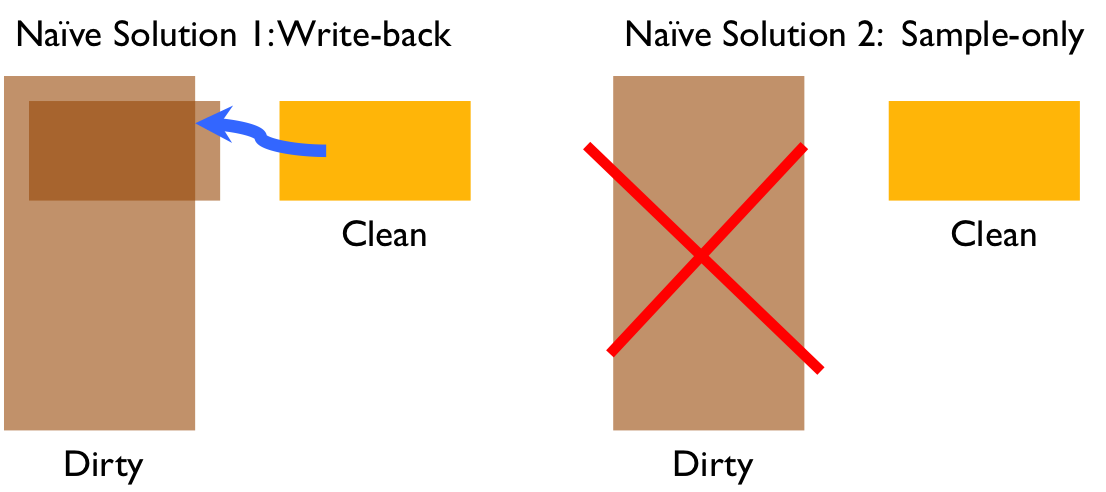
\includegraphics[width=\columnwidth]{figs/update-arch.png}
 \caption{(a) Systematic corruption in one variable can lead to a shifted model. The dirty examples are labeled 1-5 and the cleaned examples are labeled 1'-5'. 
 (b) Mixed dirty and clean data results in a less accurate model than no cleaning.
(c) Small samples of only clean data can result in similarly inaccurate models. \label{update-arch-coverletter}}
\end{figure}

\vspace{0.5em}

\noindent\textbf{R1.8 End of Sec 2.1. Why regularization term does not affect the results? It was stated w/o justification.}

\noindent We have revised the paper to make this clearer.
None of the results that we present in this paper depend on the regularization term $r(\theta)$.
Consider the regularized convex-loss minimization problem:
\[
 \theta^{*}=\arg\min_{\theta}\sum_{i=1}^{N}\phi(x_{i},y_{i},\theta) + r(\theta)
\]
Since $r(\theta)$ does not depend on on $i$, we can move it into the sum and treat is as part of $\phi$.

\vspace{0.5em}

\noindent\textbf{R1.9 Example 1 assumes very small sample (50). Why? Is that only for illustration purpose?}

\noindent   The numbers in the examples (budgets, etc.) are chosen for illustration purposes. In the particular example, each iteration samples a batch of 50 records to clean.  A discussion is included in Section \ref{sgd} on how that value can be set depending on the application:

\vspace{0.5em}
\emph{The batch size should be set by the user to have the desired properties.
Larger batches will take longer to clean and will make more progress towards the clean model but will have less frequent model updates.
On the other hand, smaller batches are cleaned faster and have more frequent model updates.}

\vspace{0.5em}

For example, if the data cleaning is implemented using crowdsourcing, then larger batches can be used. Alternatively, if the data cleaning is implemented via manual action, then smaller batches may be used.
The batch size does affect the rate of convergence, and we discuss this in Section \ref{sgd} as well. 

\vspace{0.5em}

\noindent\textbf{R1.10 Sec 4.2. Steps 4-5 need more intuition}

\noindent  Section 4.2 is Section 4.3 in the revision. We have clarified that Step 4 ``is a weighted average of the gradient on the already clean data and newly cleaned data", and Step 5 ``appends the newly cleaned data to set of previously clean records''.

\vspace{0.5em}

\noindent\textbf{R1.11 End of Sec 5. Expected Gradient Length heuristic needs more explanation}

\noindent  The discussion about Expected Gradient Length was an effort to analogize our work with Active Learning, because both are iterative algorithms. This was a side point that made the text more confusing, and we have removed it.
Section \ref{dist-samp} provides a detailed discussion of the sampling problem, what the optimal solution is, and how we apply an approximation to the optimal.

\subsection*{Review 2 Details}

\noindent\textbf{R2.1: Although the problem (iterative data cleaning) is novel, the techniques themselves are quite similar to active learning techniques.}

\noindent  We have included a revised discussion on the differences with Active Learning:

\emph{ The motivation of \sys similar to that of Active Learning~\cite{DBLP:journals/pvldb/YakoutENOI11,gokhale2014corleone} as both seek to reduce the number of queries to an analyst or a crowd.
However, Active Learning addresses a fundamentally different problem than \sys.
Active Learning poses the problem of iteratively selecting the most informative {\it unlabeled} examples to label in partially labeled datasets---these
examples are labeled by an expert and integrated into the machine learning model.
Note that Active Learning does not handle cases where the dataset is labelled incorrectly.
In contrast, \sys studies the problem of prioritizing modifications to both features and labels in existing examples.
In essence, \sys handles incorrect values in {\it any} part (label or feature) of an example.
This property fundamentally changes the type of analysis and algorithms that can be used.}

\vspace{0.5em}

\noindent\textbf{R2.2: The selection of the records to clean in each iteration (efficiency problem) uses heuristic solutions (e.g., expected gradient length). There is no formal study of the efficiency of the solution.}

\noindent  We have expanded the technical discussion of the prioritization solution and a number of experiments that evaluate its efficiency. Section \ref{dist-samp} formally describes the optimal sampling problem and our solution to it which is an approximation to the optimum. We clearly note that the \sys will converge for any sampling distribution where there is non-zero sampling probability for all remaining dirty records--and more accurate approximations only lead to faster convergence. In all of our experiments, we include ActiveClean + Oracle, which is the theoretical best performance with an optimal sampler and optimal detector.
Our results suggest that the approximate solution is very competitive to the optimum. 

 \subsection*{Reviewer 3}

\noindent\textbf{R3.1 The background sections were not very clear. This needs to be improved
to make this accessible to a general audience.}

\noindent  We have revised the background section to make the problem clearer. The background section first introduces a use case and the problems with existing tools, and then transitions to the formalism. We also significantly expanded the discussion about the system architecture~(Section \ref{syarch}), which provides intuition on the key insights.

\vspace{0.5em}

\noindent\textbf{R3.2 The jump to sampling over dirty data (Section 5.2) was too abrupt.
I do not understand statistics well enough to see why this will work at all,
and the statistically correct updates argument. Also see D6.}

\noindent  We have made several revisions to clarify the relationship between updating, sampling, and detection. We expanded the architecture section to overview the main data flows and an example of how an analyst may use \sys~(Section \ref{syarch}). Section \ref{det} now formalizes the detection component and presents our solution, and Section~\ref{dist-samp} formalizes the sampling problem and then presents our solution.

The main insight of \sys is to model the interactive data cleaning process as a form of Stochastic Gradient Descent (SGD)~\cite{bottou2012stochastic}.
SGD is an iterative optimization algorithm that starts with an initial estimate and then takes a sequence of steps ``downhill'' to minimize an objective function.
Similarly, in interactive data cleaning, the human starts with a dirty model and makes a series of cleaning decisions to improve the accuracy of the model.
We formalize the link between these two processes, and since SGD is one of the most widely studied forms of optimization, it is well understood theoretical convergence conditions.


\vspace{0.5em}

\noindent \textbf{R3.3 I was confused by Identify() in Section 2.4.
From the pseudocode, it appears Identify is picking from R,
those rows that are mispredicted under current\_model.
But why should these be the only rows that are Clean()d.
I thought cleaning was an operation that can
affect both rows that are mispredicted and rows that
are predicted correctly. Update() is not defined.}

\noindent  We have removed the pseudo-code in favor of a more precise discussion of the system architecture in Section \ref{syarch}. This new section highlights all of the components, the key data flows, and their conditions for correctness. 
The cleaning operation is applied to all rows in a batch whether or not they are predicted correctly.
In each iteration, \sys suggests a batch of data to clean based on the value to the model and the likelihood that the rows are actually dirty.

\vspace{0.5em}

\noindent \textbf{R3.4. Suppose k much less than N .. are retained .. Aren't all
the dirty records cleaned?}

\noindent This section discusses the correctness of the intermediate result (before the data are fully cleaned).
We meant to say that the user-defined cleaning function $C()$ was only applied to $k$ records.

\vspace{0.5em}

\noindent\textbf{R3.5. Sentence not clear - ' We have access to dirty
values may give us ..'}

 \noindent We have revised this to make it clear (see R2.1).

\vspace{0.5em}

\noindent\textbf{R3.6. It is not clear where R\_dirty is initialized. Do yu start with R\_dirty -= R? Or is it the set of rows misclassified in the 1st iteration?}

\noindent Section \ref{syarch} now describes the initialization as follows:

\emph{ We first initialize $R_{dirty} = R$ and $R_{clean} = \emptyset$.
The system first trains the model on $R_{dirty}$ to find an initial model $\theta^{(d)}$ that the system will subsequently improve iteratively.}

\vspace{0.5em}

\noindent\textbf{R3.7. The apriori detector assumption seems bogus.} 

\noindent  We have revised the detector section to clarify what we meant by the ``a priori'' detector (Section \ref{rule-det}). This section explains how we can integrate \emph{a priori} knowledge about which records are known to be dirty. We apologize for the lack of clarity and we have now renamed it a ``rule-based detector'' and have described concrete scenarios to which it applies. 

\vspace{0.5em}

\emph{In the data cleaning literature, error detection and error repair are treated as two distinct problems~\cite{DBLP:series/synthesis/2012Fan, Dasu:2003:EDM:861869, rahm2000data}.
Error detection is often considered to be substantially easier than error repair since one can declare a set of integrity rules on a database (e.g., an attribute must not be NULL), and select rows that violate those rules.
On the other hand, repair is harder and often requires human involvement (e.g., imputing a value for the NULL attribute).}

\vspace{0.5em}

\emph{Data quality rules are widely studied as a technique for detecting data errors.
In most rule-based frameworks, an analyst declares a set of rules $\Sigma$ and checks whether a relation $R$ satisfies those rules. The rules rules can be declared in advance before applying \sys, or constructed from the first batch of sampled data.
\sys is compatible with many commonly used classes of rules for error detection including integrity constraints (ICs), conditional functional dependencies (CFDs), and matching dependencies (MDs).
The only requirement on the rules is that there is an algorithm to enumerate the set of records that violate at least one rule.}